\documentclass[a4paper,11pt,fleqn,twoside,openright]{memoir} % Brug openright hvis chapters skal starte på højresider; openany, oneside

%%%% PACKAGES %%%%

%  Oversættelse og tegnsætning  %
\usepackage[utf8]{inputenc}					% Gør det muligt at bruge æ, ø og å i sine .tex-filer

\raggedbottom
\usepackage[all]{nowidow}
\usepackage[T1]{fontenc}  % Hjælper med orddeling ved æ, ø og å. Sætter fontene til at være ps-fonte, i stedet for bmp	
\usepackage{syntax} %til BNF
\usepackage{everyshi}
\makeatletter
\let\totalpages\relax
\newcounter{mypage}
\EveryShipout{\stepcounter{mypage}}
\AtEndDocument{\clearpage
   \immediate\write\@auxout{%
    \string\gdef\string\totalpages{\themypage}}}
\makeatother
\usepackage{longtable}
\usepackage{lscape}
\usepackage[lined,boxed,linesnumbered]{algorithm2e}
\usepackage{latexsym}										% LaTeX symboler
\usepackage{xcolor,ragged2e,fix-cm}			% Justering af elementer
\usepackage{pdfpages} % Gør det muligt at inkludere pdf-dokumenter med kommandoen \includepdf[pages={x-y}]{fil.pdf}	
\usepackage{fixltx2e}					% Retter forskellige bugs i LaTeX-kernen
\usepackage{color}
\definecolor{darkgray}{rgb}{0.95,0.95,0.95}
\usepackage{listings}
\usepackage{qtree}
\usepackage{multicol}


 \lstloadlanguages{% Check Dokumentation for further languages ...
         %[Visual]Basic
         %Pascal
         %C
	%[Sharp]C
         %C++
         %XML
         %HTML
         Java
 }
\lstset{ %
inputencoding=utf8,
literate=%
{æ}{{\ae}}1
{å}{{\aa}}1
{ø}{{\o}}1
{Æ}{{\AE}}1
{Å}{{\AA}}1
{Ø}{{\O}}1,
language=Java,                % the language of the code
basicstyle=\footnotesize\ttfamily,       % the size of the fonts that are used for the code
float = H,
xleftmargin = 10pt,
xrightmargin = 10pt,
rulecolor = \color{black},
numbers=left,                   % where to put the line-numbers
numberstyle=\footnotesize,      % the size of the fonts that are used for the line-numbers
stepnumber=1,                   % the step between two line-numbers. If it's 1, each line 
                                % will be numbered
numbersep=5pt,                  % how far the line-numbers are from the code
showspaces=false,               % show spaces adding particular underscores
showstringspaces=false,         % underline spaces within strings
showtabs=false,                 % show tabs within strings adding particular underscores
tabsize=2,                      % sets default tabsize to 2 spaces
captionpos=b,                   % sets the caption-position to bottom
breaklines=true,                % sets automatic line breaking
breakatwhitespace=false,        % sets if automatic breaks should only happen at whitespace
               % show the filename of files included with \lstinputlisting;
                                % also try caption instead of title
escapeinside={\%*}{*)},         % if you want to add a comment within your code
keywordstyle=\color[rgb]{0,0,1},
commentstyle=\color[rgb]{0.133,0.545,0.133},
stringstyle=\color[rgb]{0.627,0.126,0.941},
morekeywords={}
}

% add frame environment
\usepackage[framemethod=TikZ]{mdframed}
\mdfsetup{%
    skipbelow=\topskip,
    skipabove=\topskip,
    leftmargin=50pt,
    rightmargin=0pt,
    backgroundcolor=darkgray,
    middlelinecolor=black,
    roundcorner=10
}

\mdfdefinestyle{RoundStyle}{%
 skipbelow=\topskip,
    skipabove=\topskip,
    leftmargin=0pt,
    rightmargin=0pt,
    backgroundcolor=darkgray,
    middlelinecolor=black,
    roundcorner=10}

% needed for \lstcapt
\def\ifempty#1{\def\temparg{#1}\ifx\temparg\empty}

% make new caption command for listings
\usepackage{caption}
\newcommand{\lstcapt}[2][]{%
    \ifempty{#1}%
        \captionof{lstlisting}{#2}%
    \else%
        \captionof{lstlisting}[#1]{#2}%
    \fi%
    \vspace{0.75\baselineskip}%
}

\usepackage{tabularx}
\usepackage{changepage}

																			
%  Figurer og tabeller floats %
\pdfoptionpdfminorversion=6	% Muliggør inkludering af pdf dokumenter, af version 1.6 og højere
\usepackage{graphicx} 		% Pakke til jpeg/png billeder
\usepackage{rotating}	

%  Matematiske formler og maskinkode 
\usepackage{amsmath,amssymb,stmaryrd} 	% Bedre matematik og ekstra fonte
\usepackage{textcomp}                 	% Adgang til tekstsymboler
\usepackage{mathtools}			% Udvidelse af amsmath-pakken.
\usepackage{siunitx}			% Flot og konsistent præsentation af tal og enheder med \SI{tal}{enhed}

%  Referencer, bibtex og url'er  %
\usepackage{url}	% Til at sætte urler op med. Virker sammen med ref
%\usepackage[danish]{varioref} % Giver flere bedre mulighed for at lave krydshenvisninger
\usepackage[english]{varioref} % Giver flere bedre mulighed for at lave krydshenvisninger
\usepackage{natbib}	% Litteraturliste med forfatter-år og nummerede referencer
\usepackage{xr}		% Referencer til eksternt dokument med \externaldocument{<NAVN>}
\usepackage{nomencl}	% Pakke til at danne nomenklaturliste
\makenomenclature		% Nomenklaturliste

%  Floats  %
\let\newfloat\relax 	% Memoir har allerede defineret denne, men det gør float pakken også
\usepackage{float}
%\usepackage[footnote,draft,danish,silent,nomargin]{fixme}	% Indsæt rettelser og lignende med \fixme{...} Med final i stedet for draft, udløses en error for hver fixme, der ikke er slettet, når rapporten bygges.
\usepackage[final,silent]{fixme}
%\usepackage[draft, danish,silent]{fixme}

%%%% CUSTOM SETTINGS %%%%

%  Marginer  %
\setlrmarginsandblock{3.5cm}{2.5cm}{*}	% \setlrmarginsandblock{Indbinding}{Kant}{Ratio}
\setulmarginsandblock{2.5cm}{3.0cm}{*}	% \setulmarginsandblock{Top}{Bund}{Ratio}
\checkandfixthelayout 

%  Litteraturlisten  %
\bibpunct[,]{[}{]}{;}{a}{,}{,} 	% Definerer de 6 parametre ved Harvard henvisning (bl.a. parantestype og seperatortegn)
\bibliographystyle{bibtex/harvard}	% Udseende af litteraturlisten. Ligner dk-apali - mvh Klein

%  Indholdsfortegnelse  %
\setsecnumdepth{subsubsection}	% Dybden af nummerede overkrifter (part/chapter/section/subsection)
\maxsecnumdepth{subsubsection}	% Ændring af dokumentklassens grænse for nummereringsdybde
\settocdepth{section} 		% Dybden af indholdsfortegnelsen


%  Visuelle referencer  %
\usepackage[colorlinks, bookmarksnumbered, bookmarksdepth=4]{hyperref} % Giver mulighed for at ens referencer bliver til klikbare hyperlinks. .. [colorlinks]{..}
%\usepackage{memhfixc}
\hypersetup{pdfborder = 0 0 0}	% Fjerner ramme omkring links i fx indholsfotegnelsen og ved kildehenvisninger 
\hypersetup{			%	Opsætning af farvede hyperlinks
    colorlinks = false,
    linkcolor = black,
    anchorcolor = black,
    citecolor = black
}
\usepackage{footnote}
\makesavenoteenv{tikzpicture}

\definecolor{gray}{gray}{0.80}					% Definerer farven grå

%  Kapiteludssende  %
\definecolor{numbercolor}{gray}{0.7}			% Definerer en farve til brug til kapiteludseende
\newif\ifchapternonum

\makechapterstyle{jenor}{			% Definerer kapiteludseende -->
  \renewcommand\printchaptername{}
  \renewcommand\printchapternum{}
  \renewcommand\printchapternonum{\chapternonumtrue}
  \renewcommand\chaptitlefont{\fontfamily{pbk}\fontseries{db}\fontshape{n}\fontsize{25}{35}\selectfont\raggedleft}
  \renewcommand\chapnumfont{\fontfamily{pbk}\fontseries{m}\fontshape{n}\fontsize{1in}{0in}\selectfont\color{numbercolor}}
  \renewcommand\printchaptertitle[1]{%
    \noindent
    \ifchapternonum
    \begin{tabularx}{\textwidth}{X}
    {\let\\\newline\chaptitlefont ##1\par} 
    \end{tabularx}
    \par\vskip-2.5mm\hrule
    \else
    \begin{tabularx}{\textwidth}{Xl}
    {\parbox[b]{\linewidth}{\chaptitlefont ##1}} & \raisebox{-15pt}{\chapnumfont \thechapter}
    \end{tabularx}
    \par\vskip2mm\hrule
    \fi
  }
}			% <--

\chapterstyle{jenor}	% Valg af kapiteludseende - dette kan udskiftes efter ønske
\usepackage{wrapfig}


%\renewcommand{\headrulewidth}{0.4pt}
%\renewcommand{\footrulewidth}{0.4pt}

\usepackage{enumitem}
% Sidehoved %

\makepagestyle{custom} % Definerer sidehoved og sidefod - kan modificeres efter ønske -->
\makepsmarks{custom}{																						
\def\chaptermark##1{\markboth{\itshape\thechapter. ##1}{}} % Henter kapitlet den pågældende side hører under med kommandoen \leftmark. \itshape gør teksten kursiv
\def\sectionmark##1{\markright{\thesection. ##1}{}}	% Henter afsnittet den pågældende side hører under med kommandoen \rightmark
} % Sidetallet skrives med kommandoen \thepage	
\makeevenhead{custom}{\leftmark}{}{Group SW615F14} % Definerer lige siders sidehoved efter modellen \makeevenhead{Navn}{Venstre}{Center}{Højre}
\makeoddhead{custom}{Group SW615F14}{}{\leftmark} % Definerer ulige siders sidehoved efter modellen \makeoddhead{Navn}{Venstre}{Center}{Højre}

\usepackage{lastpage}
\usepackage{ifthen}
\usepackage{intcalc}
\usepackage{nth}

\makeevenfoot{custom}{Page \thepage}{}{Aalborg University}	% Definerer lige siders sidefod efter modellen \makeevenfoot{Navn}{Venstre}{Center}{Højre}
\makeoddfoot{custom}{Aalborg University}{}{Page \thepage}% Definerer ulige siders sidefod efter modellen \makeoddfoot{Navn}{Venstre}{Center}{Højre}		
\makeheadrule{custom}{\textwidth}{0.5pt}	 % Tilføjer en streg under sidehovedets indhold
\makefootrule{custom}{\textwidth}{0.5pt}{1mm}	% Tilføjer en streg under sidefodens indhold

\copypagestyle{nychapter}{custom} % Følgende linier sørger for, at sidefoden bibeholdes på kapitlets første side
\makeoddhead{nychapter}{Group SW615F14}{}{\leftmark}
\makeevenhead{nychapter}{Group SW615F14}{}{\leftmark}
\makeheadrule{nychapter}{\textwidth}{0pt}
\aliaspagestyle{chapter}{nychapter}	% <--
\aliaspagestyle{cleared}{custom}

\pagestyle{custom}

\usepackage{newfloat}

%%%% CUSTOM COMMANDS %%%%

\let\originaltable\table
\let\endoriginaltable\endtable
\renewenvironment{table}[1][h!t]{%
  \originaltable[#1]
  \centering}%
  {\endoriginaltable}

% Billede hack %
\newcommand{\figur}[4]{
		\begin{figure}[H] \centering
			\includegraphics[width=#1\textwidth]{billeder/#2}
			\caption{#3}\label{#4}
		\end{figure} 
}

% højrepil %
\newcommand{\ra}[0]{\rightarrow}
% epsilon %
\newcommand{\eps}{\varepsilon}

%navne macro
\usepackage{xspace}
\newcommand{\piko}{\textit{Piktooplæser}\xspace}
\newcommand{\ol}{\textit{Oasis Library}\xspace}
\newcommand{\oa}{\textit{Oasis App}\xspace}
\newcommand{\ps}{\textit{Pictosearch}\xspace}
\newcommand{\ldb}{\textit{LocalDB}\xspace}
\newcommand{\pa}{\textit{Parrot}\xspace}
\newcommand{\pt}{\textit{Piktotegner}\xspace}
\newcommand{\cat}{\textit{Kategoriværktøjet}\xspace}

% Vektor hack %
\newcommand{\vektor}[3]{
			$\begin{pmatrix}
				#1 \\ #2 \\ #3
			\end{pmatrix}$
}

% declare the floating environment {Grammar}
% this will also define \listofGrammars:
\DeclareFloatingEnvironment[
  % the file extension for the file used to create the list:
  fileext   = logr,% don't use log here!
  % the heading for the list:
  listname  = {List of Grammars},
  % the name used in captions:
  name      = Grammar,
  % the default floating parameters if the environment is used
  % without optional argument:
  placement = H
]{Grammar}

%grammatik
\newenvironment{grammatik}[2]
{
\def\fooNoI{#1} \def\fooNoII{#2}
\begin{Grammar}
\begin{grammar}
}
{
\end{grammar}
\caption{\fooNoII}\label{gra:\fooNoI}
\end{Grammar}
}

%tikz
\usepackage{tikz}
\usetikzlibrary{positioning}
\usetikzlibrary{shadows}
\usetikzlibrary{shapes,arrows}
\tikzstyle{mynodestyle} = [draw,outer sep=3,inner sep=3,minimum size=10,line width=1, very thick, draw=black!55, top color=white,bottom color=black!20]

\usetikzlibrary{arrows}
\tikzstyle{io} = [font={\bfseries},trapezium,trapezium left angle=70,trapezium right angle=-70,minimum height=0.5cm,line width=1, text=black, very thick, draw=black!55, top color=white, align=center ]
\tikzstyle{linear} = [draw, -latex']
\tikzstyle{cirkel} = [ font={\bfseries}, shape=circle, outer sep=4,minimum size=0.5cm, text=black, very thick, draw=black!55, top color=white, align=center]
\tikzstyle{cirkelgray} = [ font={\bfseries}, shape=circle, outer sep=4,minimum size=0.5cm, text=black, very thick, draw=black!55, top color=gray, align=center]
\tikzstyle{firkant} = [ font={\bfseries},outer sep=4,inner sep=7,minimum size=0.5cm,line width=1, text=black, very thick, draw=black!55, top color=white, align=center]
\tikzstyle{firkantgray} = [ font={\bfseries},outer sep=4,inner sep=7,minimum size=0.5cm,line width=1, text=black, very thick, draw=black!55, top color=gray, align=center]
\tikzstyle{tekst} = []
\tikzstyle{bendH} = [bend right=40, -triangle 60, color=red]
\tikzstyle{bendV} = [bend left=40, -triangle 60, color=red]
\tikzstyle{afrundetFirkant} = [ rounded corners ,font={\bfseries},outer sep=4,inner sep=7,minimum size=0.5cm,line width=1, text=black, very thick, draw=black!55, top color=white, align=center]
\tikzstyle{rude} = [ draw, diamond, aspect=2 ,font={\bfseries},outer sep=4,inner sep=7,minimum size=0.5cm,line width=1, text=black, very thick, draw=black!55, top color=white, align=center]
\tikzstyle{sortCirkel} = [cirkel, black, top color=black, bottom color = black]
\tikzstyle{sortCirkelPrikInner} = [cirkel, white, top color=black, bottom color = black, minimum size=0.5cm]
\tikzstyle{sortCirkelPrikOuter} = [cirkel, black, top color=white, bottom color = white, minimum size=0.7cm]
\tikzstyle{DB} = [draw=black,cylinder,shape border rotate=90,shape aspect=.25,font={\bfseries}]

%kode
\newcommand{\kode}[3]{
\noindent
\newline
\newline
\begin{minipage}{\textwidth}
\begin{mdframed}
		\lstinputlisting{kode/#3}

\end{mdframed}\lstcapt{#1}\label{lst:#2}
\end{minipage}
}

\newenvironment{code}[2]
{\def\fooNoI{#1} \def\fooNoII{#2}\noindent\newline \begin{minipage}{\textwidth}\begin{mdframed}[style=RoundStyle]}{\end{mdframed}\lstcapt{\fooNoII}\label{\fooNoI}\end{minipage}}

% quotering
\newcommand{\gaas}[{1}]{``#1''}

% lilleitem
%\newenvironment{noindlist}
 %{\vspace{-5mm}\begin{list}{\labelitemi}{\leftmargin=1em \itemindent=0em }
%\addtolength{\itemsep}{-0.5\baselineskip}}
 %{\end{list}
%\vspace{-20em}}

\newcommand{\Tau}{\mathrm{T}}

\newlist{Description}{description}{1}
\setlist[Description]{labelindent=2\parindent,leftmargin=2\parindent}

\newenvironment{inddes}
 {\begin{description}[font=$\bullet$\scshape\bfseries, labelindent=2\parindent,leftmargin=2\parindent]
 }
 {\end{description}}

\newenvironment{noindlist}
 {\vspace{-5mm}\begin{list}{\labelitemi}{\leftmargin=1em \itemindent=0em }
        \setlength{\topsep}{0pt}
        \setlength{\parskip}{0pt}
        \setlength{\partopsep}{0pt}
        \setlength{\parsep}{0pt}         
        \setlength{\itemsep}{0pt} }
 {\end{list}}

\newcommand{\doublesignaturestart}[2]{%
  \parbox{\textwidth}{
    \centering Aalborg, \today\\
    \vspace{2cm}

    \parbox{7cm}{
      \centering
      \rule{6cm}{1pt}\\
       #1 
    }
    \hfill
    \parbox{7cm}{
      \centering
      \rule{6cm}{1pt}\\
      #2
    }
  }
}

\newcommand{\longtablesetting}[1]{
\endhead
\multicolumn{#1}{c}{\textit{Continued on next page}} \\
\endfoot
\endlastfoot
}

\newcommand{\subsubsubsection}[1]{
\noindent
\textbf{#1}
}

\newcommand{\doublesignature}[2]{%
  \parbox{\textwidth}{
\vspace{2cm}
    \parbox{7cm}{
      \centering
      \rule{6cm}{1pt}\\
       #1 
    }
    \hfill
    \parbox{7cm}{
      \centering
      \rule{6cm}{1pt}\\
      #2
    }
  }
}

\newcommand{\strips}[3]{
\noindent \textbf{#1}\\
\indent \textbf{Precond:} #2\\
\indent \textbf{Effect:} #3\\\newline
}

%%%% ORDDELING %%%%

\hyphenation{hvad hvem hvor listOfErrors}
\newcolumntype{R}{>{\raggedright\arraybackslash}X}

%----------------SPROG------------------------
%----------------dk
%\usepackage[danish]{babel}							% Dansk sporg, f.eks. tabel, figur og kapitel
%\renewcommand{\algorithmcfname}{Algoritme}
%\renewcommand*{\lstlistingname}{Kodeudsnit}
%----------------en
\usepackage[english]{babel}
\usepackage{cleveref}


\usepackage{pdflscape}




%%% TO DO %%%
\usepackage[colorinlistoftodos]{todonotes}

\newcommand{\namedtodo}[5]
{
  \ifthenelse{\equal{#1}{}}
  {
    \todo[backgroundcolor=#4,caption=
    {\textbf{#3: } #2}
    ,inline]
    {\color{#5}\textbf{#3: }#2}
  }
  {
    \todo[backgroundcolor=#4,caption=
    {\textbf{#3: } #1}
    ,inline]
    {\color{#5}\textbf{#3: }#2}
  }
}
\newcommand{\Alexander}[2][]{\namedtodo{#1}{#2}{Alexander}{green}{black}}
\newcommand{\Christoffer}[2][]{\namedtodo{#1}{#2}{Christoffer}{orange}{black}}
\newcommand{\Dan}[2][]{\namedtodo{#1}{#2}{Dan}{blue!80}{white}}
\newcommand{\Kristian}[2][]{\namedtodo{#1}{#2}{Kristian}{black!10!yellow!90}{black}}
\newcommand{\Ivan}[2][]{\namedtodo{#1}{#2}{Ivan}{black!10!red!90}{white}}


  \makeatletter \renewcommand \listoftodos{\section*{List of Todos} \@starttoc{tdo}}
  \renewcommand\l@todo[2]
    {\par\noindent \textit{#2}, \parbox{10cm}{#1}\par} \makeatother

\begin{document}

% Forindhold - nummereres med romertal
\frontmatter 
\thispagestyle{empty}
\begin{flushright}
\vspace{3cm}

\phantom{hul}

\phantom{hul}

\phantom{hul}

\textsl{P8 Project} \\ \vspace{1cm}

\rule{1\textwidth}{3mm} \\ \vspace{1.5cm}
%\vspace{1cm}

\includegraphics[width=\textwidth]{Images/frontpage.jpg}
\vspace{1.5cm} \\
\textsc{\Large Tempo Player - The music player that fits YOUR tempo \\ \Ivan{Metaphor - Think about more suitable title.}
P8 Project\\
Group SW802F15\\
Software\\
Department of Computer Science\\
Aalborg University\\
Spring 2015\\
~\\
}

\end{flushright}

\cleardoublepage
\begin{nopagebreak}
	{\samepage 
		\begin{tabular}{r}
			\parbox{16cm}
			{\raisebox{11mm}
				{
\includegraphics[height=3.5cm]{Content/TitlePage/aauIcon.png}}
				\hfill \parbox{8.5cm}{\vspace{-5cm}
				\begin{tabular}{l}
					{\small \textbf{Department of Computer Science}}\\
					{\small Selma Lagerløfs Vej 300} \\
					{\small 9220 Aalborg Ø} \\
					{\small Phone (+45) 9940 9940} \\
					{\small Fax (+45) 9940 9798} \\
					{\small \url{http://www.cs.aau.dk}}
				\end{tabular}}
			}
		\end{tabular}
		
		\begin{tabular}{cc}
			\parbox{7cm}{
				\begin{description}
					\item {\textbf{Title:}} \\
						Intelligent Music with Peer-To-Peer Sharing\\
					
					\item {\textbf{Subject:}} \\
						Mobile Systems\\	
						
					\item {\textbf{Project period:}}\\
						  02-02-2015 -- 27-05-2015\\

					\item {\textbf{Project group:}}\\
						  SW802F15\\
			
					\item {\textbf{Participants:}}\\
						Alexander Drægert\\
						Christoffer\\
						Dan\\
						Kristian Thomsen \\
						  
					\item {\textbf{Supervisor:}}\\
						Ivan Aaen\\
			
					\item {\textbf{Printings:} ? }
					
					\item { \textbf{Pages:} ?? }
					 
					\item { \textbf{Appendices:} ? }
					
					\item { \textbf{Total pages:} ?? }
					
					\item { \textbf{Source code:}\\ 
					{\small \mbox{\footnotesize\url{https://github.com/SW802F15/SourceCode/tree/???????}}}}
			
				\end{description}
				\vfill 
			}
			&	 
			\parbox{6cm}{
				\hfill \\ \\
				\begin{tabular}{l}
					{Abstract:\smallskip}\\ 
					\fbox{
						\parbox{6cm}{
							\bigskip{
								\vfill
								{\small 
									This report contains
Lorem ipsum dolor sit amet, consectetur adipiscing elit. Cras consectetur tristique justo, vel pellentesque augue porttitor ut. Suspendisse potenti. Aliquam ipsum metus, commodo eget eros eu, consectetur auctor turpis. Suspendisse potenti. Sed ut felis elit. Proin eget urna placerat ante rutrum scelerisque ac id neque. Quisque gravida porttitor pulvinar. Fusce feugiat arcu at quam hendrerit, nec ultrices dui fermentum. Nam non nibh ac ligula suscipit dictum. Ut sit amet massa at massa ornare lobortis et ac neque. Duis vulputate mauris sit amet dictum iaculis. Praesent tellus velit, lobortis ac elit in, laoreet efficitur tortor. Etiam blandit, mi ac tincidunt tincidunt, ante sapien efficitur leo, eu efficitur nisi elit condimentum sem. Mauris vulputate neque ut lorem consequat semper. Praesent non tempus tellus.
									\smallskip
								}
							}
						}
					}
				\end{tabular}
			}
		\end{tabular}
		\\ \\
	}
\noindent{\footnotesize\emph{The content of the report is freely available, but may only be published (with source reference) with consent from the authors.}}
\end{nopagebreak}
\cleardoublepage
\chapter{Preface}


















~\\\\
\doublesignaturestart{Alexander Drægert}{Christoffer N'Dûru}
\doublesignature{Dan Petersen}{Kristian Thomsen}
\cleardoublepage

% Indholdsfortegnelse (TOC)
\setlength\parskip{0ex} % Fjerner den vertikale afstand mellem hver linie i indholdsfortegnelse
\tableofcontents* % Indholdsfortegnelsen 
\setlength{\parskip}{3mm} % Aktiverer afstanden igen for resten af rapporten (afstem med preamble!)
%\addtocontents{toc}{\protect\newpage} % Fremtvinger sideskift i indholdsfortegnelsen hvis nødvendig


 % Hovedindhold - nummereres fra side 1
\mainmatter
\makeevenfoot{custom}{Page \thepage~of \pageref{LastPage}}{}{Aalborg University} % Definerer lige siders sidefod efter modellen \makeevenfoot{Navn}{Venstre}{Center}{Højre}
\makeoddfoot{custom}{Aalborg University}{}{Page \thepage~of \pageref{LastPage}} % Definerer ulige siders sidefod efter modellen \makeoddfoot{Navn}{Venstre}{Center}{Højre}		
\pagestyle{custom}

% Rapportindhold
\chapter{Introduction}
\label{chap:intro}
%First Problem - Idea Domain%
Running is a popular form of exercise, however, it can be a tedious and uninspiring endeavour.
To improve the experience, \citet{musicRunEffectArticle} found that 
\textit{``... participants enjoyed what they were doing [running] more when they were listening to music of any sort when compared to when they were not.''}

It was further concluded by \citet{musicRunEffectArticle} that the volume and tempo of the music influenced the running experience.
They concluded that the running pace for novice runners, while listening to relatively low-tempo music, was slower than when not listening to music. Additionally listening to high-tempo music resulted in a faster running pace, compared to when not listening to music.

This conclusion is in disagreement with the conclusion of \citet{musicNoPerformanceEffect} which suggests, that \textit{``... music had no impact on mean power output.''}. \citet{musicNoPerformanceEffect} measure the running pace by mean power output, nevertheless, they did not see any impact on the running pace by listening to music.

As a result, we can not definitively conclude whether music of different tempo will affect the running experience differently. 
However by adhering to \citet{musicRunEffectArticle}'s conclusion, we can only improve the running experience, since \citet{musicNoPerformanceEffect} concludes there can be no negative impact, by playing music.

Today many runners use their smartphone as a music player, which can either be placed in their hand, pocket, or on their arm.
The sensors in a smartphone enable monitoring the pace and speed of the runner.
Based on this knowledge the first problem can be stated:

\begin{center}
\textit{How can we provide music with an appropriate tempo, compared to the current pace, to the runner through the use of a smartphone?}
\end{center}

%Second Problem - UI%
\noindent Operating a smartphone while running is difficult, especially if it is placed in the pocket or on the arm of the runner.
In order for the runner to operate the smartphone; play, pause, stop, or change song, the runner would have to stop running, or focus more than normally. This can disrupt the runner's form, and lead to injuries and accidents.
Based on this knowledge the second problem can be stated: 

\begin{center}
\textit{How can a smartphone application be operated without disrupting the runner's form and/or concentration?}
\end{center}
%Third Problem - Methodology%
%\noindent Most large scale software projects fail. 
\noindent According to \citet{gartner:failure} \textit{``A full 66 percent of large scale projects fail ...”}, and although this is not a large scale project, some of the same pitfalls exist.
One way to avoid some of these pitfalls, is \textit{``... using a structured systems development methodology ...”}, since it according to \citet{dorsey:methodologyReason} \textit{``... is one of the critical success factors in a systems development project.”}.

We will in this project focus on the development methodology \texttt{Extreme Programming} (XP).
XP is used because its an interesting methodology and it is development oriented.
Furthermore, XP's requirements of self-organising teams, iteration length, and team size fit well with this project. 
Based on this knowledge the third problem can be stated:

\begin{center}
	\textit{How do we adapt the structured systems development methodology, Extreme Programming, to our project?}
\end{center}

\chapter{Analysis}
\label{chap:analysis}
\section{Problem Domain}
\section{Problem Statement}
Running is a popular form of exercise, however it can be a tedious and uninspiring endeavour.
To improve the experience, \citet{musicRunEffectArticle} found that 
\textit{``... participants enjoyed what they were doing [running] more when they were listening to music of any sort when compared to when they were not.''}

It was further discovered by \citet{musicRunEffectArticle} that the volume and tempo of the music influenced the running experience.
They discovered that the running speed, while listening to relatively slow music, was slower than when not listening to music. Additionally listening to fast-paced music resulted in a faster running speed, compared to when not listening to music.

Today many runners use their smartphone as a music player, which can either be placed on their arm or in their pocket.
The sensors in a smartphone allows for reading the steps per minute and speed of the runner.

\begin{center}
\textit{How can this data be used and calculated upon to provide the runner with an enjoyable running experience?}
\end{center}

\Ivan{Will the app follow the users tempo or will the user follow the music?}
\Ivan{Think about and discuss difference types of running e.g. interval.}
\Ivan{Maybe have options to choose between 3 mode: plain (music follows user), fast (user follows music), interval or other template (user follows music of different BPM).}

With a smartphone placed on their arm or in their pocket, it is difficult to navigate applications through visual feedback. Furthermore operating the smartphone while running decreases the navigability of the smartphone. \Alexander{SOURCE} 
The runner's form should not be disrupted by navigating. 
\Alexander{Re-write last (previous $\uparrow$) line.}

\begin{center}
\textit{How can a smartphone application be operated without disrupting the runner's form?}
\end{center}


\chapter{Methodology}
\label{chap:methodology}
\Alexander{Check and Correct used time - past-tense vs. future-tense vs. etc}
\section{Extreme Programming}
XP (Extreme Programming) is an agile development methodology. This project will be developed while using the principles of XP.

\subsection{Motivation}
XP follow 12 principles.\Alexander{Source to Beck Book+}

These 12 principles should ease the development of high quality software.
This is partly done by ensuring thorough testing, continuously refactoring, and efficient knowledge sharing.
XP further encourages improving oneself and the teams as a whole.
This is partly done by pair programming, sprint reviews, and collaborative ownership.

For these principles to work there are some criteria there needs to be met, some of those criteria are:
\begin{itemize}
\item The size of an XP team should not exceed ten members.
\item Iterations should not exceed four weeks, but two-three weeks are preferable.
\item The team should be self-organising and should not be controlled by a boss.
\item The team members must be able to embrace change.
\item The team should have their workstations placed in the same room.
\end{itemize}

All the listed criteria is fulfilled by this project.

\subsection{Approach}
According to \citet[p. 53]{xp:explained}, the idea behind these practices is that while one practice in itself is weak, the others can cover that weakness. This creates a synergy effect between the practices. This also means that if one or more of the practices are chosen to be discontinued or modified, careful consideration should be made.

%Continued practices
We have chosen to adopt 8 of the 12 practices. 
The adopted practices in this project are:
\begin{itemize}
\item Small Releases
\item Simple Design
\item Testing
\item Refactoring
\item Pair Programming
\item Collective Ownership
\item Continuous integration
\item 40-hour Work Week
\end{itemize}

\paragraph{Testing} will be implemented by writing unit tests and acceptance tests before writing any production code. After the tests and production code is written, they will be run frequently to ensure that everything is working as it is specified, especially after adding new features to the system.

\paragraph{Refactoring} will be implemented by team members making changes where they are needed. Also, code standards will be discussed and adhered to. Pair Programing also aids refactoring since two people programming together will be more likely to have the courage to refactor difficult pieces of code. The Testing practice also aids in this since tests can be run after refactoring which lessens the possibility of the code breaking.

%\paragraph{Small Releases} have been implemented by releasing new, working features with small increments, every iteration consisting of around two weeks.

%\paragraph{Simple Design}\Christoffer{What should we do about this?}

%Discontinued practices
The practices that have been discontinued are:
\begin{itemize}
\item The Planning Game
\item Metaphor
\item On-site Costumer
\item Coding Standards
\end{itemize}

\paragraph{Planning Game} has been discontinued in favour of Planning Poker as described by \citet{xp:planningPoker}.\Christoffer{do we follow this completely?}
The main difference is how conflicting estimations are resolved.
Planning Poker starts with the team discussing the task. This ensures everybody understand the scope and task at hand. This will in-turn reduce disparity of the individual estimates, and make it easier to agree on an estimate. Each member then considers his estimate and keeps it to himself. When all are ready, everybody reveals their estimate at the same time. If there is great disparity between estimates, a discussion is organised. When this discussion is over, everybody estimates the task again. If the conflict still exists, the estimate is decided by ``Optimism wins''.
\Alexander{Find where the source concludes this.}

The Planning Game starts with the team discussing the task. Then each member considers his estimate and reports this to the team. If a conflict have aroused, estimation are chosen by ``Optimism wins'' as stated by \citet[p. 58]{xp:planning}.
This way of reporting individual estimates may influence the estimation of other team member. 
 \Alexander{Explained p.153 description of individual version of planning game (should be used?).
			Planning p.58 description of collaborative version of planning game (used in report).
			We originally chose Poker Planning because we only knew the individual version of Planning Game.}
 \Alexander{Explained p.157, Planning game not necessary four teams of 3-4 developers.}
 

\paragraph{Metaphors} have not been implemented, since we find the product simple enough to understand without any metaphors. 

\paragraph{On-site Costumer} have not been possible to implement, since we do not have a costumer. We have therefore decided to act as our own on-site costumer.
\Alexander{Should be re-written!}

\paragraph{Coding Standards} have not been implemented. Although general guidelines are adhered to.
\Alexander{Should be elaborated upon.}

\chapter{Step Counter}
\label{chap:stepCounter}
In the following sections, the development of our step counter module will be explained.
\Christoffer{Intro omskrives?}
\section{User Stories}
\subsection{Step Counter}
\story{Detect the pace of the user.}{High}
{As a user, I, want the application to detect my pace and display it on the screen. }
{\begin{itemize}
\item When I run the screen displays my SPM.
\end{itemize}}

\story{Select song based on pace.}{High}
{As a user, I, want the application to select song to play based on my pace.}
{\begin{itemize}
\item When I run the application automatically selects songs matching my pace.
\end{itemize}}
\section{Specification}

\section{Implementation}
The Step counter is implemented as a single class extending the \texttt{Service} class in Android. The service is started and bound from the \texttt{MusicPlayerActivity}, meaning in our implementation it is launched and closed together with the \texttt{MusicPlayerActivity}. On its creation the \texttt{StepCounterService} registers the accelerometer sensor in order to read data required for step detection.


\subsection{Step Detection}\label{sec:stepCnt}
To determine whether a step is taken, the approach taken by \citet{zhao:pedometer} is implemented. Our implementation first calculates a threshold, which corresponds to the threshold line in \Cref{fig:zhaoGraph}. The threshold is calculated by subtracting the minimum accelerometer measurement from maximum measurement, from the array where the measurements are stored.

According to \citet[p. 2]{zhao:pedometer} a step has occurred if there is a negative slope in the acceleration graph and the acceleration curve crosses the threshold. It is determined whether a negative slope has occurred, by comparing the latest accelerometer measurement with the previous one. If the last measurement was above the threshold, and the current is below the threshold, a negative slope which crossed the threshold and thus, a step has occurred.

As \citet[p. 2]{zhao:pedometer} we assume that a person can either run as fast as five steps per second or walk as slowly as one step every two seconds. This is handled in the implementation by checking the time since the last measurement. If less than 200 milliseconds have passed since the last step, a new step is not detected. If more than 2 seconds have passed the SPM array is updated with a 0 to indicate that the person is not moving (0 steps per minute).

Our implementation utilises an sensitivity limit so measurements which are very close to each other are not detected as a new step, even though they fulfill the requirements mentioned earlier. This is done to filter out small deviations in measurements which might falsely be identified as a new step. The current limit value is 2, and was found experimentally.
\begin{figure}[h!]
  \centering
    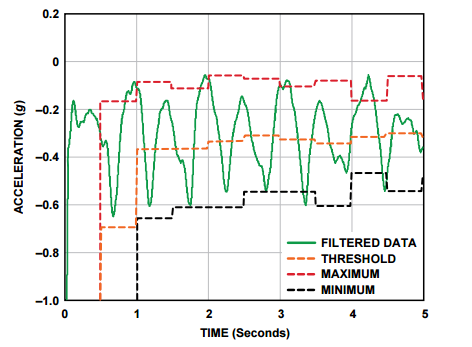
\includegraphics[scale=0.8]{Images/accPlot.png}
  \caption{An acceleration plot from \citet[p. 2]{zhao:pedometer} showing filtered data from a pedometer worn by a person walking.}
  \label{fig:zhaoGraph}
\end{figure}


\subsection{Calculation of Steps Per Minute}
The gab between steps are used to calculate the number of steps the user takes per minute (SPM).

First, the amplitude is calculated which represents the change x, y, z values obtained from the accelerometer. The formula used for this is $$amplitude = \sqrt{x^{2} + y^{2} + z^{2}}$$

The array containing accelerometer measurement data is then updated with the newly calculated value. The data in this array is used for determining whether a step is taken or not, the implementation of which is described in \Cref{sec:stepCnt}.

If we detect a step we look when the previous step was taken and calculate SPM from that, this value is then stored in the array containing the SPM measurements. Afterwards, the average value of the SPM array with the new value is calculated, and the GUI is updated with a new value through a GUI manager.

If no step is taken and more than 2 seconds have passed, the implementation interprets this as if no steps are being taken and the SPM array and GUI is updated with the value 0.

\chapter{Conclusion}
\label{chap:conclusion}
\section{Discussion}
\section{Future Work}
\subsection{Application}
% interval programs
% offline analysis
	% minor since we are customers. Why?
% online album cover
% adjust music speed
% integration with music streaming service
% settings should be expanded
	% editing of songs (IDx-tags (bpm etc.))
	% what more?
% fix cover flow
% head phone in / out
% fixed play
% true NGUI
% tactile feedback

\subsection{Extreme Programming}
% determine long-term effect of having a coding standard
%test
	% mutation test
% have customer available

\section{Conclusion}

%\clearforchapter
\appendix	% Appendiks/bilag start - giver chapter bogstaver i stedet for talf
\addtocontents{toc}{\protect\cftpagenumbersoff{chapter}} % Fjernelse af nummerering af bilag i TOC
\settocdepth{chapter}	% Sætter dybden af indholdsfortegnelsen til chapter for bilagene

%%%% Appendiks %%%%
\clearforchapter
\begin{vplace}[0.7]
\begin{center}
\Huge \textbf{Appendix}
\end{center}
\end{vplace}















\chapter{Project CD}
\label{chap:dvd}
The CD found on this page contains the following:
\begin{itemize}
\item The source code for 
\item A compiled version of 
\item A digital version of the report in PDF format.
\end{itemize}


\bibliography{Bibliography/bibliography}




%%% DELETE BEFORE FINAL %%%
\chapter{Examples \& ToDo}
\Alexander{Example of comment/ToDo made by Alexander}

\Christoffer{Example of comment/ToDo made by Christoffer}

\Dan{Example of comment/ToDo made by Dan}

\Kristian{Example of comment/ToDo made by Kristian}

\Ivan{Example of comment/ToDo made by Ivan}

\begin{code}{lst:label}{Caption of code snippet}
\begin{lstlisting}
public class HelloWorld {

    public static void main(String[] args) {
        System.out.println("Hello, World");
    }

}
\end{lstlisting}
\end{code}

This is how you refer to a source written by \cite{Test}.
\clearpage
\listoftodos
\end{document}